\pdfobjcompresslevel=1
\documentclass[10pt]{beamer}

% In general, you should encode all files using UTF-8
\usepackage[utf8]{inputenc}
\usepackage[T1]{fontenc}

% Include SIunits to get \unit for unit typesetting
\usepackage[squaren]{SIunits}
% Set the math mode font to sans-serif
\let\mathrm\mathsf

% If you are not using SLC5/6 (or for any other reason pdfTeX before 1.40.6)
% you may comment this line. This just fixes transparent images with
% pdfs when viewed with acrobat reader and compiled with old versions of
% pdfTeX.
\pdfpageattr {/Group << /S /Transparency /I true /CS /DeviceRGB>>}

% Use this for better font scaling (esp. if you want to use \tiny)
\usepackage{lmodern}
\usepackage{exscale}

% You can safely remove this package, it is just for displaying a layout
% page
\usepackage{layout}

% Enable rounded corners for standard blocks:
% \setbeamertemplate{blocks}[rounded]

% Add some paragraph spacing:
%\setlength{\parskip}{\smallskipamount} 

\usepackage{listings}
\lstset{
  language={C},
  basicstyle={\small}}


\title{Pthreads (POSIX Threads)}
\date{Practical Course on Parallel Computing
Apr., 2018}
\author[Practial Course on Parallel Computing - Pthreads]{Dr. Gen Kawamura\\ \small{ATLAS Experiment, A. Quadt}}
\institute[2. Physik]{II. Physikalisches Institut, Georg-August-Universit\"at G\"ottingen}


\usetheme{ugoe}

\def\insertlogos{%
  
\includegraphics[height=1.2cm]{logos/BMBF-Gef-Logo}%
  \hspace{1cm}%
  
\includegraphics[height=1.2cm]{logos/FSP103}%
  \hspace{1cm}%
}

% Alternative logo sizes / order
%\def\insertlogos{%
%   
\includegraphics[height=2cm]{logos/logo-uni-goe-notext.pdf}%
%   \hspace{0.1cm}%
%   \includegraphics[height=1.5cm]{logos/FSP101-Atlas-Logo}%
%   \hspace{0.1cm}%
%   
\includegraphics[height=1.5cm]{logos/BMBF-Gef-Logo}%
%   \hspace{0.1cm}%
%   \includegraphics[height=2cm]{logos/helmholtz_logo}%
%}

\AtBeginSection[]{\begin{frame}\frametitle{Table of Contents}\tableofcontents[currentsection]\end{frame}}
\begin{document}

% Title
\begin{frame}
  \titlepage
\end{frame}

% List of Contents
\begin{frame}
\begin{columns}
        \column{0.7\textwidth}
        \tableofcontents
        \column{0.2\textwidth}
        \vspace{-2cm}\hspace{-2cm}\reflectbox{
\includegraphics[width=1.2\textwidth]{pictures/magic.png}}
\end{columns}
\end{frame}


% --------------------------------------
% Processes and Threads
% --------------------------------------
\section{Processes and Threads}

% Processes
\subsection{Processes}

\begin{frame}
        \frametitle{Excursion: Processes}
        \begin{itemize}
                \item Common operating systems on common hardware handle a lot of \emph{processes} at once
                \item Each one with it's own set of \emph{virtual memory}
                \item All processes are strictly separated for security, simplicity and compatibility reasons
                \item Each \emph{core} can only run one process at a time
                \item At different intervals the \emph{scheduler} stops the process, changes the memory-Content of the CPU core (aka \emph{the registers}) and starts another one.
        \end{itemize}
\end{frame}


\begin{frame}
        \frametitle{Excursion: Processes \#2}
        \vspace{0.5cm}
        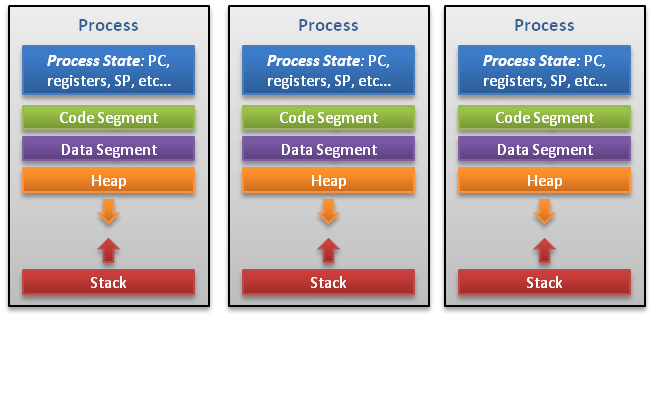
\includegraphics[width=0.7\textwidth]{pictures/process_no_sm.png} \\
        \vspace{-0.5cm}
        {\footnotesize \hspace{3cm}Memory structure of a process on a common Operating System/ CPU architecture}        
\end{frame}


\begin{frame}
        \frametitle{Multiple Core / Shared Memory Systems}
        \vspace{0.5cm}
        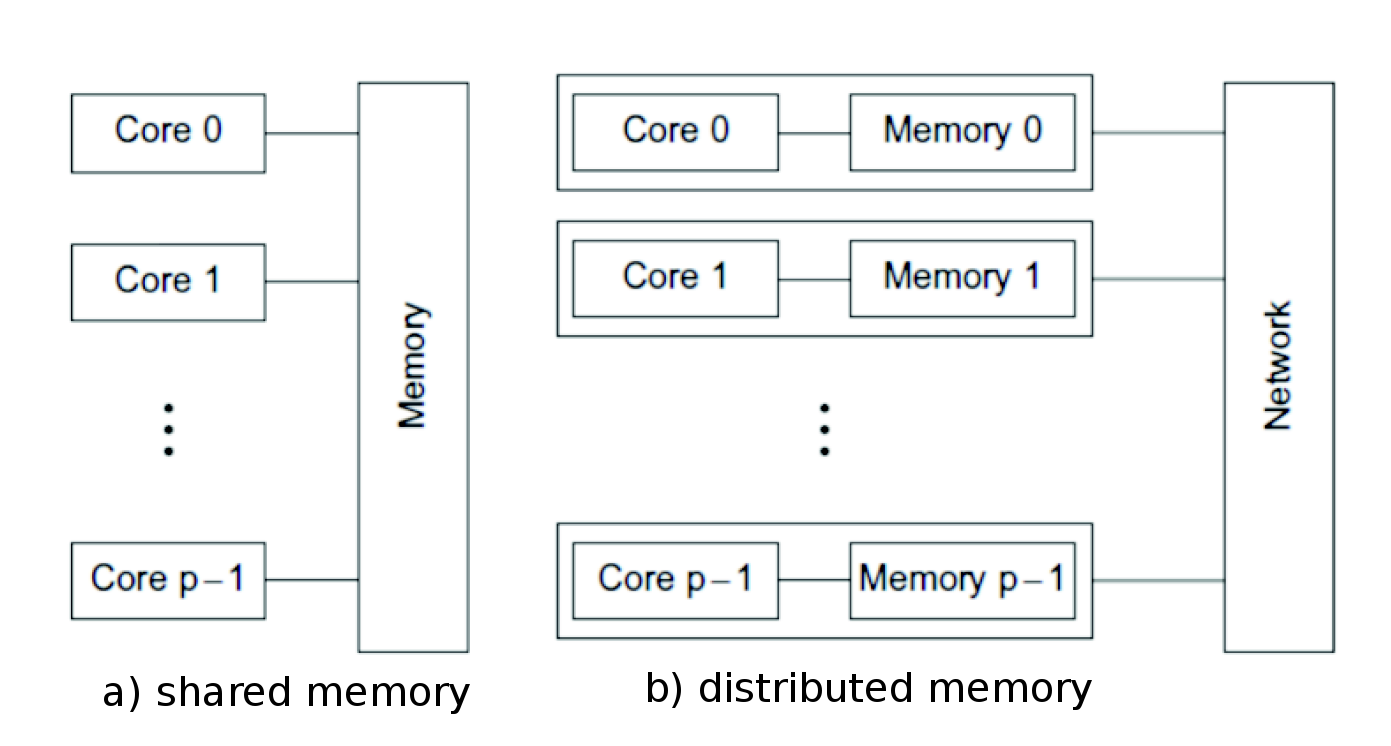
\includegraphics[width=\textwidth]{pictures/smdm.png} \\
        %\vspace{0.5cm}
        %{\footnotesize \hspace{3cm}(a) Shared memory\hspace{2cm} (b) Distributed Memory}
\end{frame}


\begin{frame}
        \frametitle{Multiple Core / Shared Memory Systems \#2}
        \begin{itemize}
                \item Run one program per CPU core simultaneously
                \begin{itemize}
                        \item Start one process which sets up the environment
                        \item and spawns one worker-process per core via fork(3)
                \end{itemize}
                \item Idea: Communicate via inter-process (shared) memory
                \item But $\ldots$
                \begin{itemize}
                        \item Memory from different processes strictly separated (on common OS)
                        \item How to deal with simultaneous access on same memory page?
                \end{itemize}
        \end{itemize}
\end{frame}


% Threads
\subsection{Threads}
        
\begin{frame}
        \frametitle{Threads as a lightweight alternative}
        \begin{itemize}
                \item Idea for SMP machines: separate the state and stack but share the heap
                \item \emph{Lightweight Process} or \emph{Thread}
        \end{itemize}
                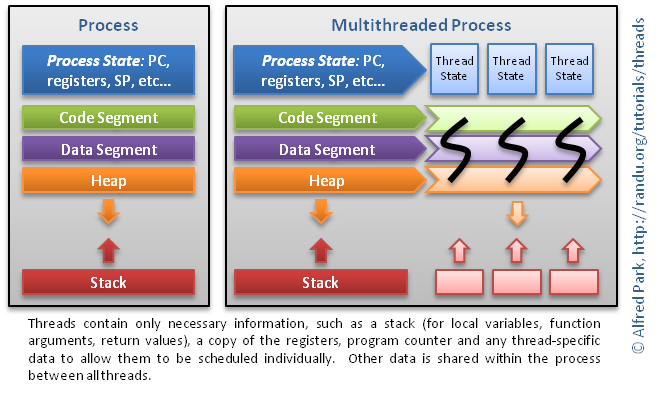
\includegraphics[width=0.7\textwidth]{pictures/process.png}
\end{frame}


\begin{frame}
        \frametitle{Very short Operating System intermezzo}
        \begin{itemize}
                \item How does the OS scheduler handle threads?
                \begin{itemize}
                        \item 1:1 i.e. one thread is one \emph{job} in the scheduler. The case for most recent OS
                        \item n:1 or n:m i.e. multiple threads are mapped to one \emph{job}. In this case the library or even the threads have to schedule themselves
                \end{itemize}
                \item One might compare the 2 models above with preemptive vs. cooperative scheduling or with kernel- vs. user-(space)-threads.
        \end{itemize}
\end{frame}

\begin{frame}
        \frametitle{How to \emph{create} Threads}
        \begin{itemize}
                \item Linux: clone (2) system call; implemented in the NPTL-lib (and glibc)
                \item Mac OS X: NSThread class (from Cocoa)
                \item Windows: CreateThread() library call
                \item POSIX Threads: \emph{pthreads}
                \begin{itemize}
                        \item most Unix': Linux, Mac OS X, Solaris, BSDs$\ldots$ 
                        \item even on Windows
                \end{itemize}
                \item And many abstractions like boost, QT, glib etc.
        \end{itemize}
\end{frame}

\begin{frame}
        \frametitle{We will use POSIX Threads (pthreads)}
        \begin{itemize}
                \item Set of (c-) library functions in pthread.h
                \item Abstracts the underlying OS
                \item Provides very basic functionality but everything needed to start 
                \item If using frameworks like QT one should use their implementations.
                \item For C++ one can use the language inherent std::thread class (since C++11)
                \item C version 11 also has standard threads.h but this is not widely implemented  
        \end{itemize}
\end{frame}

\begin{frame}
        \frametitle{In the following}
        \begin{itemize}
                \item $\ldots$we will have a close look at some of pthreads features
                \item $\ldots$we will learn about general concepts of multi-threading
        \end{itemize}
\end{frame}


% ==========================================
%  POSIX Threads
% ==========================================
\section{POSIX Threads}

%----------------------
% General Concepts
%----------------------
\subsection{General Concepts}
\begin{frame}[fragile]
\frametitle{General Concepts}
\begin{itemize}
        \item Not all features are available on all systems
        \item You only deal with functions
        \item If you want to change data objects you have to (!) use special functions
\end{itemize}

% https://qiita.com/ayihis@github/items/c779e4ab5cd7580f1f87
\begin{block}{Working with pthreads}
\begin{lstlisting}
#include <pthread.h>
pthread_t thread;
// Create attribute object
pthread_attr_t attr;
// Initialize it
pthread_attr_init(&attr);
// Change it
pthread_attr_setdetachstate(&attr, PTHREAD_CREATE_JOINABLE);
// use it
r = pthread_create(&thread, &attr, [...]);
\end{lstlisting}
\end{block}
\end{frame}


\begin{frame}[fragile]
	\frametitle{Most basic program}
\begin{block}{Basis}
\begin{lstlisting}
//compile with   gcc -pthread basic.c
#include <stdio.h>
#include <pthread.h>
void *hello()
{
    printf("Hello World.\n");
    pthread_exit(NULL);
}
main () {
    pthread_t thread;
    pthread_create(&thread, NULL, hello, NULL);
    pthread_exit(0);
}
\end{lstlisting}
\end{block}
\end{frame}

%----------------------
% Create, Exit and Cancel Threads
%----------------------
\subsection{Create, Exit and Cancel Threads}

\begin{frame}
	\frametitle{Create, Exit and Cancel Threads}
	\begin{itemize}
		\item A thread is terminated if
		\begin{itemize}
			\item the function ends
			\item it calls {\it pthread\_exit}(int return\_value)
			\item it gets killed with {\it pthread\_cancel}(thread\_id)
			\item main() ends without waiting (it might wait with {\it pthread\_exit})
			\item the process is terminated/ killed by the OS
		\end{itemize}
		\item {\it pthread\_exit} does not clean after itself -- you have to free() memory, close files etc.
	\end{itemize}
\end{frame}


\begin{frame}
	\frametitle{A short word on scheduling}
	\begin{itemize}
		\item On Linux you can change the scheduling parameters via setpriority (2), pthread\_setaffinity\_np (3) or sched\_setaffinity (2).
		\item This might be important for binding on a specific core on NUMA machines.
	\end{itemize}
\end{frame}



\begin{frame}[fragile]
	\frametitle{Passing arguments}
\begin{block}{With arguments}
\begin{lstlisting}
void *answer(void *value)
{
    long number = (long) value;
    printf("The answer is %ld.\n", number);
    pthread_exit(NULL);
}
int main () {
    long value = 42;
    pthread_t thread;
    pthread_create(&thread, NULL, answer, (void *) value);
    pthread_exit(0);
}
\end{lstlisting}
\end{block}
\end{frame}


\begin{frame}
	\frametitle{Passing many arguments}
\begin{block}{With arguments}
Read hello\_arg2.c
\end{block}
\end{frame}

\begin{frame}
    \frametitle{Wait for another thread}
    \begin{itemize}
        \item {\it pthread\_join}(threadid, status) -- waits for thread {\it threadid} and writes the {\it pthread\_exit} return code into {\it status}
        \item A thread can only be joined by {\emph exactly one} other thread
        \item Example later!
    \end{itemize}
    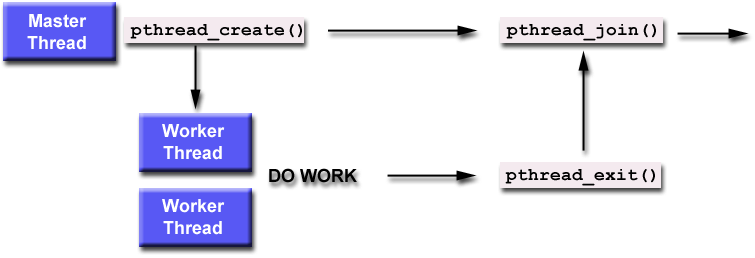
\includegraphics[width=0.8\textwidth]{pictures/joining.png}
\end{frame}


%----------------------
% Shared Data
%----------------------
\subsection{Shared Data}

\begin{frame}[fragile]
	\frametitle{Shared and Distributed Data}
	\begin{itemize}
		    \item Global C variables are global over thread boundaries
		    \item Memory in heap ({\it malloc}) is global over threads boundaries
		    \item Variables in stack are {\emph non}-global
		\end{itemize}
%		\begin{snugshade}
\begin{block}{Shared Data with a pointer}
\begin{lstlisting}
int global_variable=42;
int main() {
    int non_global_variable=23;
    int *pointer_to_global_data = malloc(sizeof(int));
    [...]
}
\end{lstlisting}
\end{block}
\end{frame}


\begin{frame}[fragile]
\frametitle{Basic Example for shared data}
\begin{block}{Basic Example}
\begin{lstlisting}
int answer=42;
void *hello()
{
    printf("The answer is again %d\n",answer);
}
int main () {
    pthread_t thread;
    pthread_create(&thread, NULL, hello, NULL);
    pthread_create(&thread, NULL, hello, NULL);
    pthread_exit(0);
}
\end{lstlisting}
\end{block}
\end{frame}



%----------------------
% Locking Data
%----------------------
\subsection{Locking Data}

\begin{frame}[fragile]
    \frametitle{Locking Data}
    \begin{itemize}
        \item pthread offers a native Mutex implementation
        \item A Mutex shields a part of code. Once you are in this code no one else can go into it.
        \item Syntacticly a Mutex is a set of functions and a data object
    \end{itemize}

\begin{block}{}
\begin{lstlisting}
mutex_t mymutex;
void thread_1() {
[...]
    lock(mymutex);      // as long as mymutex is locked
        do_something(); // no one else can lock it
    unlock(mymutex);
[...]
}
void thread_2() {
[...]
    lock(mymutex);      // so thread_2 might have to wait
        do_something_else();
    unlock(mymutex);
[...] }
\end{lstlisting}
\end{block}
\end{frame}


\begin{frame}
    \frametitle{pthread Mutex functions}
    \begin{itemize}
\item {\it pthread\_mutex\_t} -- mutex data structure
\item {\it pthread\_mutex\_init}(mutex, NULL) -- initialize mutex variable
\item {\it pthread\_mutex\_destroy}(mutex) -- destroy it
\item {\it pthread\_mutex\_lock}(mutex) -- lock the mutex; will block and stop the thread until mutex is available
\item {\it pthread\_mutex\_unlock}(mutex) -- can only be called by the mutex-owning thread
\item {\it pthread\_mutex\_trylock}(mutex) -- lock the mutex but does not block; might return with a \emph{impossible-to-lock} error code
    \end{itemize}
\end{frame}

\begin{frame}
    \frametitle{Example for the use of a mutex}
    dotprod\_serial.c \\
    dotprod\_mutex.c
\end{frame}

\begin{frame}
    \frametitle{Some considerations}
    \begin{itemize}
        \item A mutex does no magic! The one and only function is to block until the owner unlocks it.
        \item Think of it as a gentleman's agreement.
        \item The scheduling is non-deterministic! Any thread might get the lock first! Beware of deadlocks!!
    \end{itemize}
\end{frame}

\begin{frame}
    \frametitle{A word on semaphores}
    \begin{itemize}
        \item a semaphore is similar to a mutex but it \emph{counts} the number of lock holders
        \item pthread does not offer a native semaphore type!
        \item but {\it semaphore.h} does.
        \item c.f. sem\_init (3)
    \end{itemize}
\end{frame}



%----------------------
% Signaling and 
% Condigion Variables
%----------------------
\subsection{Signaling and Condition Variables}
    

\begin{frame}[fragile]
    \frametitle{Signaling and Condition Variables}
    \begin{itemize}
        \item With a condition variable we can signal another thread about an event, e.g. that we are finished doing something.
    \end{itemize}
\begin{block}{}
\begin{lstlisting}
physics() {
    calculate_gravity();
    signal_ready(physics);
    [...] }
artifical_intelligence() {
    look_around();
    move_oponents();
    signal_ready(ai):
    [...] }
game(){
    for_each_timestep {
        [...]
        wait_for(physics);
        wait_for(ai);
        paint_graphics();
        }
}
\end{lstlisting}
\end{block}
\end{frame}


\begin{frame}
    \frametitle{Conditions with pthreads}
    \begin{itemize}
    \item {\it pthread\_cond\_t} -- data structure
\item {\it pthread\_cond\_init}(condition, NULL)
\item {\it pthread\_cond\_destroy}(condition)
\item {\it pthread\_cond\_wait}(condition, mutex) -- wait for condition {\it condition}
\item {\it pthread\_cond\_signal}(condition) -- signal to one thread only that the {\it condition} is fullfilled
\item {\it pthread\_cond\_broadcast}(condition)  -- signal to EVERYBODY that the {\it condition} is fullfilled
    \end{itemize}
\end{frame}


\begin{frame}
    \frametitle{Using conditions with pthreads}
    \begin{itemize}
        \item You always need an additional mutex to shield the condition!
        \item {\it cond\_wait}(cond, mutex)
        \begin{itemize}
            \item should be called after {\it mutex} is locked by the same thread!
            \item \emph{unlocks} {\it mutex} and blocks
            \item waits for the {\it cond} to be signaled
            \item unblocks and immediately \emph{locks} {\it mutex}
            \item You have to unlock the {\it mutex} afterwards!
        \end{itemize}
        \item The thread might wake up from {\it cond\_wait} although the condition is not fulfilled! $\rightarrow$ You should put it inside a {\it while}-loop.
        \item If there is the smallest possibility that more then one thread waits for a condition -- use {\it cond\_broadcast}!
    \end{itemize}
\end{frame}


\begin{frame}
    \frametitle{Example for Conditions}
    condvar.c
\end{frame}


\begin{frame}[fragile]
    \frametitle{Barriers}
    \begin{itemize}
        \item A barrier is a construct to synchronize threads
        \item All threads that arrive at a barrier have to wait until everybody else is there
        \item When initializing we have to specify the maximum number of threads that have to wait
    \end{itemize}

\begin{block}{}
\begin{lstlisting}
mybarrier = barrier(9); // we have 8 planets and one sun

calc_planet_position (my_planet) {
    while (true) {
        calc_force_on_my_planet(all_planet_positions);
        move_my_planet();
        
        //wait for the other planets to finish
        barrier_wait(mybarrier);
    }
}
\end{lstlisting}
\end{block}
\end{frame}


\begin{frame}
    \frametitle{Barriers in pthread}
    \begin{itemize}
    \item \texttt{pthread\_barrier\_t} -- data type
        \item {\it pthread\_barrier\_init}(barrier, attr,number) -- initialize new barrier which stops {\it number} of threads
        \item {\it pthread\_barrier\_wait}(barrier) -- blocks until {\it number} threads called this function
        \item {\it pthread\_barrier\_destroy}(barrier) 
    \end{itemize}
\end{frame}

%\begin{frame}
%    \frametitle{Example of a Barrier}
%    barrier.c
%\end{frame}


% ==========================================
%  Performance Considerations
% ==========================================

\section{Performance}


%----------------------
% Performance Consideration
%----------------------
\subsection{Performance Considerations}  
\begin{frame}
        \frametitle{Performance Considerations}
        \begin{itemize}
            \item \emph{Lock granularity} -- How coarse or fine are your mutexes? Do they lock a whole structure or fields of a structure? The more fine-grained, the more concurrency you can gain.
            \item \emph{Lock frequency} - Are you locking (too) often? Locking at unnecessary times? Reduce such occurrences to fully exploit concurrency and reduce synchronization overhead.
            \item \emph{Critical sections} - You should minimize critical sections i.e. section that can only be entered by one thread at a time.
            \item \emph{Worker thread pool} - If you are using a Boss/Worker thread model, make sure you pre-allocate your threads instead of creating threads on demand.
            \item \emph{Too many threads?} - At what point are there too many threads? Can it severely impact and degrade performance?
        \end{itemize}
\end{frame}


%----------------------
% Bug and Performance Example
%----------------------
\subsection{Bug and Performance Example}
\begin{frame}
    \frametitle{Bug and Performance Example}
    bug6.c \\
    bug6\_correct.c
\end{frame}


\begin{frame}[fragile]
    \frametitle{Example for a Deadlock}
\begin{columns}
        \column{0.5\textwidth}
\begin{block}{Thread 1}
\begin{lstlisting}
pthread_mutex_lock(&m1);
/* use resource 1 */ 

pthread_mutex_lock(&m2);

/* use resources1 and 2 */ 


pthread_mutex_unlock(&m2);
pthread_mutex_unlock(&m1); 
\end{lstlisting}
\end{block}

        \column{0.5\textwidth}

\begin{block}{Thread 2}
\begin{lstlisting}
pthread_mutex_lock(&m2);
/* use resource 2 */ 

pthread_mutex_lock(&m1);

/* use resources 1 and 2 */ 


pthread_mutex_unlock(&m1);
pthread_mutex_unlock(&m2); 
\end{lstlisting}
\end{block}
\end{columns}
\end{frame}


%----------------------
% Conclusioon
%----------------------
\section{Conclusion}
\begin{frame}
    \frametitle{Conclusion}
    \begin{itemize}
        \item Threads are a nice way to parallelize problems on a shared memory architecture
        \item pthreads offer an OS abstraction for threads, mutexe and signal handling (conditions and barriers)
        \item Avoid race conditions but also avoid deadlocks.
    \end{itemize}
\end{frame}

\begin{frame}
    \frametitle{Literature}
    \begin{itemize}
        \item pthreads (7) man page and pthread\_* (3) man pages
        \item \url{http://pages.cs.wisc.edu/~travitch/pthreads_primer.html}
        \item \url{http://randu.org/tutorials/threads/}
        \item \url{https://computing.llnl.gov/tutorials/pthreads/} (also has a reference)
        \item Practical Course on Parallel Computing - Sose2015 (The most content/codes were from this material)
    \end{itemize}
\end{frame}


\begin{frame}
\frametitle{Questions}
\begin{center}

\includegraphics[width=0.5\textwidth]{pictures/questions.png}
\end{center}
\end{frame}


\end{document}
